% 静电的基本规律和性质
% 电磁学-静电基本现象和规律|库仑定律

\subsubsection{两种电荷}
\footnote{参考: 新概念物理教程 电磁学(赵凯华, 陈熙谋)}高中时候我们就已经了解到摩擦带电,并且人们将用绸子摩擦过的玻璃棒所带电荷称为正电荷,将用毛皮摩擦过的硬橡胶棒所带电荷叫做负电荷.(注意这种命名一开始是任意的,但一直沿用至今)

这两种电荷相互接触能够互相中和,也就是正负电荷完全抵消.

\textbf{性质} 同性相斥,异性相吸.(也就是同种电荷相互排斥,异种电荷相互吸引)

\subsubsection{电荷守恒定律}
电荷既不能被创造,也不能被消灭,它们只能从一个物体转移到另一个物体,或者从物体的一部分转移到另一部分.换句话说,就是任何物理过程中电荷的代数和是守恒的.(这是物理学中的普遍的基本定律)
\begin{equation}
\sum Q_i=C
\end{equation}

\subsubsection{电荷的量子化(charge quantization)}
 通过密里根油滴实验,密里根发现油滴所带的总电荷是一个数值的整数倍.这个数值就是电荷量$e$,也就是量子化的.
 在这里稍微提一下其实验内容, 对其实验感兴趣的读者可以去查找相关资料作为补充阅读.

具体实验图如下:

\begin{figure}[ht]
\centering
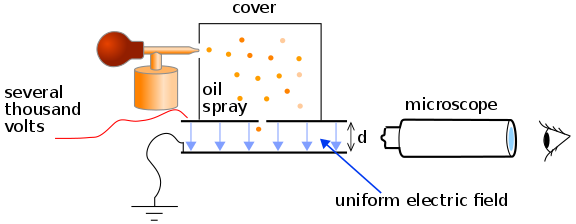
\includegraphics[width=12cm]{./figures/EM1_2.png}
\caption{Simplified scheme of Millikan's oil drop experiment(来自维基百科)} \label{EM1_fig1}
\end{figure}

这个实验的原理是根据油滴的受力平衡原理(粗略的理解可以认为:油滴的重力$mg$和电场力$qE$平衡,但其实具体实验过程中还需考虑空气的粘滞性对油滴产生的阻力等因素),计算出油滴的带电量,从而得出电荷量.)

\subsubsection{点电荷}

在研究带电体的时候,当带电体的形状大小,和电荷分布等因素可以忽略不考虑的情况下,我们为了研究的方便,经常把这样的物体抽象的看成一个几何点,也就是点电荷.

% 还有其他性质为补充完全